% !TEX TS-program = lualatex
% !TEX encoding = UTF-8

% This is a  template for creating an oversize initial in gregorio + latex.

\documentclass[12pt]{article} % use larger type; default would be 10pt
\usepackage{geometry} % See geometry.pdf to learn the layout options. There are lots.
\geometry{a4paper} % or letterpaper (US) or a5paper or....
\usepackage{gregoriotex} % for gregorio score inclusion
\usepackage{fullpage} % to reduce the margins
\usepackage[oldstyle]{libertine} % a font I like
\usepackage{lettrine} %for big initials in text outside of the chant scores
\usepackage{titlesec} %change the look of titles
\usepackage{graphicx}

% red colour
\definecolor{benred8}{HTML}{E82C00}

% FORMAT SUBSUBSECTIONS - use titlesec package
\titleformat{\subsubsection}{\centering\normalfont\color{benred8}}{}{1em}{}
\titlespacing{\subsubsection}{0 mm}{0 mm}{0 mm}

% SPACE BETWEEN Capitulum AND BIBLE VERSE
\def\capitulumSpace{\hspace{20 mm}}

% MAKES Ps : TEXT
\def\psalm{\textit{\textcolor{benred8}{Ps :}}}

% MAKES ALL \gresixstars RED
\let\oldgresixstar\gresixstar
\renewcommand{\gresixstar}{\textcolor{benred8}{\oldgresixstar}}

% MAKES ALL \gredaggers RED
\let\oldgredagger\gredagger
\renewcommand{\gredagger}{\textcolor{benred8}{\oldgredagger}}

% MAKES ALL \Vbars RED
\let\oldVbar\Vbar
\def\VVbar{\textcolor{benred8}{\oldVbar\oldVbar .}}
\renewcommand{\Vbar}{\textcolor{benred8}{\oldVbar .}}

% MAKES ALL \Rbars RED
\let\oldRbar\Rbar
\renewcommand{\Rbar}{\textcolor{benred8}{\oldRbar .}}

% MAKES ALL \Abars RED
\let\oldAbar\Abar
\renewcommand{\Abar}{\textcolor{benred8}{\oldAbar .}}

% MAKES T.P. TEXT
\def\TemporePaschale{\textit{\textcolor{benred8}{T. P.}}}

% RESPONSE ENVIRONMENT
\newenvironment{response}{\leftskip 0in \setlength{\parindent}{0in}}{\vspace{2 mm}}

\begin{document}

\pagestyle{empty}

\begin{center}

	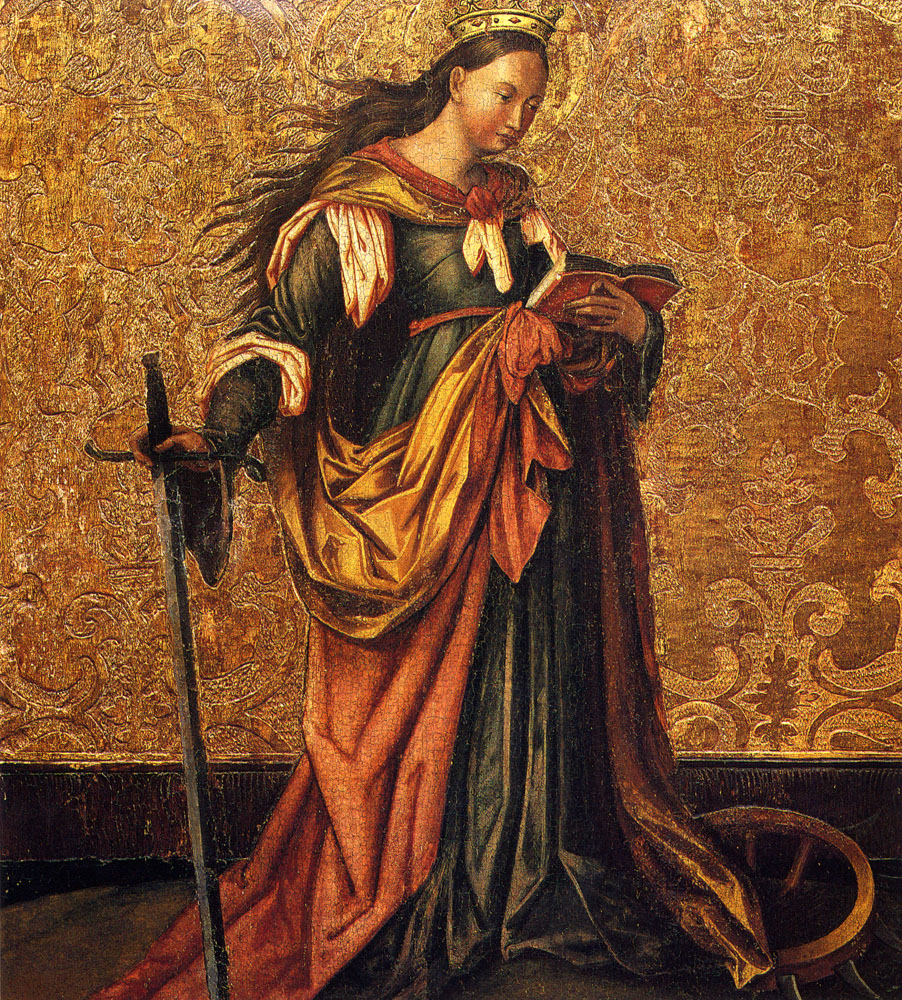
\includegraphics[width=10cm]{st-catherine-of-alexandria.jpg}
	
	\vspace*{5.0mm}

	\begin{Large}\textsc{\textcolor{benred8}{Commemoratio de Sancta Catharina.}}\end{Large}

\end{center}

% Here we set the space around the initial.
% Please report to http://home.gna.org/gregorio/gregoriotex/details for more details and options
\setspaceafterinitial{2.2mm plus 0em minus 0em}
\setspacebeforeinitial{2.2mm plus 0em minus 0em}

% Here we set the initial font. Change 43 if you want a bigger initial.
\def\greinitialformat#1{%
{\fontsize{43}{43}\selectfont #1}%
}

% Here we set the oversize initial font.
\def\grebiginitialformat#1{%
{\fontsize{120}{120}\selectfont #1}%
}

% We set IV above the initial. Had to adjust position a bit with \raisebox:
\gresetfirstlineaboveinitial{\raisebox{-0.30cm}{\textcolor{benred8}{\small \textsc{\textbf{I}}}}}{}

%\gresetfirstlineaboveinitial{\textcolor{benred8}{\small \textsc{\textbf{IV}}}}{}

%%%%%%%%%%%%%%%%%%%%
% ADJUSTING THE POSITION OF THE INITIAL
% FROM INSIDE resurrexi_score.tex :
% NORMALLY:
% \greinitial{R}%
% REPLACED WITH:
% \raisebox{0.70cm}{\greinitial{R}}%
%%%%%%%%%%%%%%%%%%%%


\includescore{virgosanctacatharina_score.tex}

\begin{response}
\Vbar\ Diff\'{u}sa est gr\'{a}tia in labiis tuis.

\Rbar\ Propt\'{e}rea bened\'{i}xit te Deus in \ae t\'{e}rnum.

\end{response}

\subsubsection*{\textcolor{black}{Or\'{e}mus.}\capitulumSpace \emph{Oratio.}}

\begin{response}\lettrine{D}{e}us, qui ded\'{i}sti Legem Moysi in summit\'{a}te montis S\'{i}nai, et in e\'{o}dem loco per sanctos Angelos tuos corpus be\'{a}t\ae\ Cathar\'{i}n\ae\ V\'{i}rginis et M\'{a}rtyris tu\ae\ mirab\'{i}liter colloc\'{a}sti~:~\gresixstar\ pr\ae sta, qu\'{\ae}sumus ; ut ejus m\'{e}ritis et intercessi\'{o}ne, ad montem qui Christus est perven\'{i}re vale\'{a}mus. Qui tecum vivit et regnat in unit\'{a}te Sp\'{i}ritus Sancti Deus, per \'{o}mnia s\'{\ae}cula s\ae cul\'{o}rum. \Rbar\ Amen.

\end{response}


%\begin{center}\begin{Large}\textsc{\textcolor{benred8}{Gradual.}}\end{Large}\end{center}

% We set IV above the initial.
%\gresetfirstlineaboveinitial{\textcolor{benred8}{\small \textsc{\textbf{II}}}}{\textcolor{benred8}{\small \textsc{\textbf{II}}}}

%\includescore{haec_dies_score.tex}

\end{document}